\documentclass[12 pt]{article}
\usepackage[utf8]{inputenc}
\usepackage{amsmath,amssymb,graphicx,amsthm,float}
\usepackage{xcolor,soul,tikz}

\usetikzlibrary[cd]
\usepackage[left=3cm,right=3cm,top=3cm,bottom=3.5cm]{geometry}


\usepackage{mathtools}
\usepackage{tikz}
\usetikzlibrary{shapes,snakes}
\usepackage[shortlabels]{enumitem}

\usepackage{stackengine}
\newcommand\bracecirc[1]{%
  \ensurestackMath{\stackengine{-2pt}
  {\aoverbrace[L1R]{#1}}{\scriptstyle\circ}{O}{c}{F}{F}{S}}%
}

\RequirePackage[colorlinks=true,
    pdfstartview=FitV,
    linkcolor=blue,
    citecolor=blue,
    urlcolor=blue,
    breaklinks=true,
    pdfencoding=auto,
    hyperfootnotes=false]{hyperref}

\RequirePackage{aliascnt}
\RequirePackage{amsthm,amssymb,amsmath}
\RequirePackage{cleveref}

\newtheorem{theorem}{Theorem}[section]
    \crefformat{theorem}{\bfseries theorem~#2#1#3}
    \Crefformat{theorem}{\bfseries Theorem~#2#1#3}
\newtheorem{corollary}[theorem]{Corollary}
    \crefformat{corollary}{\bfseries corollary~#2#1#3}
    \Crefformat{corollary}{\bfseries Corollary~#2#1#3}
\newtheorem{lemma}[theorem]{Lemma}
    \crefformat{lemma}{\bfseries lemma~#2#1#3}
    \Crefformat{lemma}{\bfseries Lemma~#2#1#3}
\newtheorem{prop}[theorem]{Proposition}
    \crefformat{prop}{\bfseries proposition~#2#1#3}
    \Crefformat{prop}{\bfseries Proposition~#2#1#3}
    
\theoremstyle{definition}
\newaliascnt{defn}{theorem}
\newtheorem{defn}[theorem]{Definition}
    \crefformat{defn}{\bfseries definition~#2#1#3}
    \Crefformat{defn}{\bfseries Definition~#2#1#3}
\newtheorem{remark}[theorem]{Remark}
\newtheorem{exa}[theorem]{Example}
    \crefformat{exa}{\bfseries example~#2#1#3}
    \Crefformat{exa}{\bfseries Example~#2#1#3}

\newtheorem*{xrem}{Remark}
\newcommand{\DMO}[1]{\DeclareMathOperator{#1}}

\newcommand{\R}{\mathbb{R}}
\newcommand{\N}{\mathbb{N}}
\newcommand{\Z}{\mathbb{Z}}
\newcommand{\C}{\mathbb{C}}
\newcommand{\Q}{\mathbb{Q}}
\newcommand{\E}{\mathbb{E}}
\newcommand{\calE}{\mathcal{E}}
\DeclareMathOperator{\Bun}{Bun}
\newcommand{\ang}[1]{\left\langle #1\right\rangle}
\newcommand{\ceil}[1]{\left\lceil#1\right\rceil}
\newcommand{\floor}[1]{\left\lfloor#1\right\rfloor}
\DMO{\im}{im}
\DMO{\id}{id}
\newcommand{\inc}{\xhookrightarrow{}}
\newcommand{\iso}{\xrightarrow{\sim}}
\DMO{\Hom}{Hom}
\DMO{\coker}{coker}
\DMO{\Ext}{Ext}
\newcommand{\ol}[1]{\overline{#1}}
\newcommand{\Hc}[1]{H_{\text{c}}^{#1}}
\newcommand{\Hgp}[1]{H_{\text{gp}}^{#1}}
\newcommand{\bbS}{\mathbb{S}}

\title{}

\date{}

\begin{document}

\section{Introduction}

Let $G$ be a group and $A$ a right $G$-module. It is well-known that the second group cohomology $\Hgp2(G;A)$ is in natural correspondence with the group $\E(G;A)$ of (equivalence classes of) extensions of $G$ by $A$. Topologically, it is also known that $\Hgp2(G;A)$ is in natural correspondence with $H^2(BG;A)$, the singular cohomology of $BG$ with local $A$-coefficients. Hence, we obtain a natural correspondence
\begin{equation}\label{classical deg2}
\E(G;A)\iso H^2(BG;A).
\end{equation}
In this project, we construct and study a natural map
$$\alpha:\E(G;A)\to [BG,(B^2A)_{hG}]_{BG}$$
which is defined when $G$ and $A$ are topological groups (with mild niceness assumptions) with $G$ acting continuously on $A$, such that $\alpha$ agrees with the classical isomorphism when $G$ and $A$ are discrete. Here, $\E(G;A)$ denotes the group of (equivalence classes of) those extensions of $G$ by $A$ which are also locally trivial principal $A$-bundles. $[BG,(B^2A)_{hG}]_{BG}$ is the group of homotopy classes of sections of the projection $(B^2A)_{hG}\to BG$, where $(B^2A)_{hG}$ denotes the homotopy $G$-orbit space of $B^2A$. When $A$ is discrete, this naturally agrees with singular cohomology with local $A$-coefficients:
$$[BG,(B^nA)_{hG}]_{BG}\cong H^n(BG;A).$$

The motivation behind this project is two-fold. First observe that in the classical case, the definition of the map \eqref{classical deg2} goes through group cohomology. Working with topological groups forces one to instead use more direct topological insights to construct and study the map, hence providing new topological insight for what initially seems like an algebraic coincidence. Second, the map $\alpha$ can be thought of as assigning to each extension a characteristic class, hence allowing the use of homotopy-theoretic tools in the study of such extensions.

\subsection{The case of simple coefficients}

It turns out that $\alpha$ is not a bijection in general, e.g the Heisenberg group $H$ is a non-trivial central extension of $G=\R^2$ by $A=\R$, but $[BG,(B^2A)_{hG}]_{BG}=0$ since $BG$ is contractible. See \S10.2 of \cite{Ja} for an example where surjectivity fails. However, we show that a coarser notion of surjectivity does hold when $G$ acts trivially on $A$:

\begin{theorem}\label{essential surjectivity}
Suppose $G$ acts trivially on $A$. There exists a CW group $G'$ and a homotopy equivalence $G'\to G$ which is also a group homomorphism such that $\alpha:\E(G';A)\to H^2(BG';A)$ is surjective.
\end{theorem}

Combining this with Theorem 1.1 of \cite{JJS} yields

\begin{theorem}\label{essential bijectivity}
Suppose $G$ acts trivially on $A$ and $A$ is discrete. There exists a CW group $G'$ and a homotopy equivalence $G'\to G$ which is also a group homomorphism such that $\alpha:\E(G';A)\to H^2(BG';A)$ is an isomorphism.
\end{theorem}

For the case of $G$ acting non-trivially on $A$, we believe that `injectivity up to homotopy' results can be obtained using similar techniques as those used in \cite{Ja}; we plan to pursue these during Round 2. Additionally, we can answer Question 10.3.2 of \cite{Ja} in the positive using the techniques used to define $\alpha$.

\subsection{Agreement with the classical map}
As in \cite{Ja, JJS}, our definition of $\alpha$ is non-constructive — it relies on an existence argument using properties of classifying spaces. In \Cref{G A discrete}, we construct a zig-zag which allows us to obtain a concrete formula for $\alpha$ on $B_2G$, the second element of the skeletal filtration of the Milgram--Steenrod construction. This technique is similar to the one used in \cite{Ja} for the case of simple coefficients, but a different zig-zag construction is required for non-simple coefficients. Hence, we obtain

\begin{theorem}\label{(thm) G A discrete}
When $G$ and $A$ are discrete, the composition
$$\E(G;A)\overset{\alpha}{\to}[BG, (B^2A)_{hG}]_{BG}\iso H^2(BG;A)$$
agrees with the classical isomorphism $\E(G;A)\cong H^2(BG;A)$.
\end{theorem}

\subsection{Original mathematical contributions in Round 1}
All the results in this report were proved during the 40 hours of Round 1, and only the open weight models provided by Open Math OS were used for AI assistance in producing these proofs (see \Cref{documentation} and \Cref{formalization section} for details on the AI use for the documentation and Lean formalization). All of the numbered results in this report are original work, although we drew heavily on \cite{Ja, JJS} for the big-picture ideas. Many of the questions we answer here were first raised in \cite{Ja}.


\section{Notation and convention}
We follow \cite{Ja} for conventions related to compactly generated spaces and the definitions of CW groups and $k$-groups. For $G$ a CW group and $A$ an abelian $k$-group, we say that $A$ is a (right) $G$-module if there is a continuous map $A\times G\to A$ satisfying the obvious relations.

We use $B$ and $E$ to denote the Milgram--Steenrod construction of the classifying space and universal space respectively; see \S2.2 in \cite{Ja} for the relevant properties and conventions. For any space $X$ with a continuous right $G$-action, we write $X_{hG}$ for the Borel construction of the homotopy orbit space of $X$, which is the orbit space of the diagonal $G$-action on $EG\times X$.

\begin{lemma}\label{hom orb}
There is a natural homeomorphism
$$B(G\ltimes A)\cong (BA)_{hG}.$$
\end{lemma}

\begin{proof}
Let $p:G\ltimes A\to G$ be the projection and consider the map $\phi:E(G\ltimes A)\to EA$ given by the formula
\begin{equation}\label{E(semi-dir)}
\phi\left(\prod_{i=1}^n(g_i,a_i,t_i)\right)=\left(\prod_{i=1}^n(a_i\cdot(g_{i+1}\dots g_n),t_i)\right).
\end{equation}
One checks that $\phi$ is well-defined and $(G\ltimes A)$-equivariant. Hence, $Ep\times \phi:E(G\ltimes A)\to EG\times EA$ is also $(G\ltimes A)$-equivariant, and has a continuous inverse. Taking the quotient by the $(G\ltimes A)$-action yields the desired homeomorphism.
\end{proof}

\begin{remark}
The well-definedness calculation required for the above proof were formally verified in Lean; see \Cref{formalization section}.
\end{remark}

Henceforth, we will treat the above homeomorphisms $B(G\ltimes A)\cong (BA)_{hG}$ and $E(G\ltimes A)\cong EG\times EA$ as identifications. Note that $(BA)_{hG}\to BG$ is a group bundle with fiber group $BA$; fiber-wise multiplication and inversion are descended from the trivial group bundle $EG\times EA\to EG$ with fiber group $EA$.


\section{Topological abelian group extensions}
Let $G$ be a CW group and let $A$ be an abelian topological group with a continuous right $G$-action via group homomorphisms. 
An extension of $G$ by $A$ is a short exact sequence
$$\calE: 1\to A \to E \to G \to 1$$
of groups which is a principal $A$-bundle and respects the action of $G$ on $A$.
Write $\E(G;A)$ for the group (under Baer sums) of equivalence classes of such extensions.

Given $\calE\in\E(G;A)$, we obtain a $G$-equivariant principal $BA$-bundle
$$BA\to EE/A \to EG,$$
i.e., the $G$- and $BA$-actions satisfy
$$(x\cdot z)\cdot g=x\cdot(z\cdot g)$$
for $x\in EE/A$, $g\in G$, and $z\in BA$. The underlying principal $(G\ltimes BA)$-bundle yields a class $\alpha(\calE)\in [BG, B(G\ltimes BA)]_{BG}$. By \Cref{hom orb}, this defines a map
$$\alpha:\E(G;A)\to [BG, (B^2A)_{hG}]_{BG}$$
Since $(B^2A)_{hG}\to BG$ is an abelian group bundle, $[BG, (B^2A)_{hG}]_{BG}$ is an abelian group and $\alpha$ is a homomorphism. Write $F$ for the forgetful map
$$\E(G;A)\to\Bun_G(A)$$
which remembers only the principal $A$-bundle structure underlying an extension.

\begin{prop}\label{bundle str}
$\ker\alpha\subset\ker F$, i.e., $\alpha$ detects the underlying bundle structure of extensions. 
\end{prop}

\begin{proof}
Let $\calE\in\ker\alpha$. Hence, as a $(G\ltimes BA)$-principal bundle, $EE/A \to BG$ is the push-forward of the universal $G$-bundle along the projection $G\ltimes BA\to G$. Hence, the inclusion $\iota:G\inc G\ltimes BA\inc EE/A$ factors through $EG\inc EE/A$. Since $EG$ is contractible, this shows that $\iota$ is null-homotopic. However, the pull-back of the principal $A$-bundle $EE\to EE/A$ along $\iota$ is $F(\calE)$,\footnote{In fact, the same is true at the level of group extensions by $A$.} so $\calE\in\ker T$.
\end{proof}

\section{Essential surjectivity of $\alpha$ for simple coefficients}

Which classes in $[BG,(B^2A)_{hG}]_{BG}$ come from an abelian group extension, i.e., what is the image of $\alpha$? This is a hard question to answer for a general pair $(G,A)$, but it turns out that $\alpha$ is surjective in a coarser sense when $G$ acts trivially on $A$; this is \Cref{essential surjectivity}.

\begin{proof}[Proof of \Cref{essential surjectivity}]
Let $\bbS:\textbf{Top}\to \textbf{sSet}$ denote the simplicial complex functor, and similarly let $\bbS_\ast:\textbf{Top}_\ast\to\textbf{sSet}_0$ denote the reduced simplicial complex functor. Write $\mathbb{G}:\textbf{sSet}_0\to \textbf{sGrp}$ for Kan's loop-group functor and $\bar W:\textbf{sGrp}\to\textbf{sSet}_0$ for its right-adjoint. Let $X=\bar W\bbS G$ and $\mathcal{A}=\bbS A$. Note that $\bar W$ takes $\textbf{sAb}$ to $\textbf{sAb}$, so $\bar W^2\mathcal{A}$ makes sense. Recall that
\begin{itemize}
\item for any space $Y$, evaluation gives a weak equivalence $|\bbS Y|\to Y$, and the restriction $|\bbS_\ast Y|\to Y$ is also a weak equivalence if $Y$ is based and connected,
\item $|X|\simeq BG$ and the counit $\mathbb{G}X\to \bbS G$ is a weak equivalence, and similarly\\
\item $|\bar W^2\mathcal{A}|\simeq B^2A$. 
\end{itemize}

Pick a class $\zeta\in H^2(BG;A)$, and let $f:X\to\bar{W}^2\mathcal{A}$ be a simplicial representative ($f$ exists since $\bar W^2\cal A$ is a Kan complex). The adjoint $\hat{f}:\mathbb{G}X\to\bar{W}\mathcal{A}$ is a simplicial group homomorphism, so pulling back the simplicial central extension
$$\mathcal{A}\to W\mathcal{A}\to \bar{W}\mathcal{A}$$
along $\hat{f}$ gives a simplicial central extension
$$\mathcal{A}\to \mathcal{E}\to \mathbb{G}X.$$
Finally, we set $G'=|\mathbb{G}X|$ push the above central extension forward along the evaluation map $|\mathcal{A}|\to A$ to get the desired preimage of $\zeta$ in $\E(G',A)$. The desired homotopy equivalence $G'\to G$ is given by $G'\to\bbS G\to G$ (it is clear that this is a weak equivalence, and then we use the fact that $G'$ and $G$ are both CW complexes). 
\end{proof}

\section{$\alpha$ when $G$ and $A$ are discrete}\label{G A discrete}

Recall the construction of the continuous group cohomology $\Hc{\ast}(G;A)$ from \S2.4 of \cite{Ja}; this generalizes immediately to the present context of $G$ acting non-trivially on $A$. The correspondence $T:\Hc2(G;A)\iso\ker F$ from \S2.5 of \cite{Ja} also holds (this is the continuous analogue of the classical correspondence between second group cohomology and abelian group extensions for discrete groups).

For $f:G^{\wedge2}\to A$ a normalized continuous 2-cocycle, we wish to describe $\alpha T(f)$ explicitly in terms of $f$.

\begin{theorem}\label{alpha_2}
The image of $\alpha T(f)$ under the restriction
$$[BG, (B^2A)_{hG}]_{BG}\to[B_2G, (B^2A)_{hG}]_{BG}$$
is represented by the formula
$$\Phi_f:(\vec{g},\vec{t})\mapsto \left((\vec{g},\vec{t}),(f(\vec{g}),\eta_2(\vec{t})\right).$$
\end{theorem}

\begin{proof}[Sketch of proof of \Cref{(thm) G A discrete}]
Follow the argument from \S5.3 of \cite{Ja} by analogy — cellular cohomology of $BG$ with simple $A$-coefficients is replaced by its local coefficient analogue, and $[BG, B^2A]$ is replaced by $[BG, (B^2A)]_{BG}$. Just as the formula in \cite{Ja}, the above formula extends to a unique section $BG\to (B^2A)_{hG}$ up to homotopy for dimensional reasons, and this unique extension is $\alpha(f)$.
\end{proof}

Let $\calE=T(f)$. To prove \Cref{alpha_2}, we construct a zigzag of continuous group morphisms
\begin{equation}\label{zigzag}
% https://tikzcd.yichuanshen.de/#N4Igdg9gJgpgziAXAbVABwnAlgFyxMJZABgBpiBdUkANwEMAbAVxiRAHEQBfU9TXfIRQBGclVqMWbADrS8DWAAJOPPtjwEiAJjHV6zVog6yGeALbxFAIQCC3cTCgBzeEVAAzAE4QzSUSBwIJDIJAxlpNCwQagY6ACMYBgAFfg0hEE8sJwALHG5eEC8fP2pApB1QqSNZAGs6NDQ6ey4gA
\begin{tikzcd}
G & \tilde G \arrow[l, "\pi"'] \arrow[r, "\kappa"] & G\ltimes BA
\end{tikzcd}
\end{equation}
such that $\pi$ is a homotopy equivalence and
\begin{equation}\label{Bzigzag}
% https://tikzcd.yichuanshen.de/#N4Igdg9gJgpgziAXAbVABwnAlgFyxMJZABgBpiBdUkANwEMAbAVxiRACEBxEAX1PUy58hFAEZyVWoxZt2AHTl4GsAATc+A7HgJEATBOr1mrRBwAUnBQzwBbeCvYBBAJS9JMKAHN4RUADMAJwgbJDIQHAgkfRAAIxgwKCQAZjCGOjiGAAVBbREQBhg-HBBDaRMQBUY0AAs6MwUAY0YAUVcNEEDgpHFwyMRdds6QxB6I0J4KHiA
\begin{tikzcd}
BG \arrow[rr, "\alpha(\calE)", bend left] & B\tilde G \arrow[r,"B\kappa"] \arrow[l,"B\pi"'] & B(G\ltimes BA)
\end{tikzcd}
\end{equation}
commutes up to homotopy.

\begin{remark}
The zig-zag involving $X_\calE:=EE/A$ used to prove Theorem 5.2.1 of \cite{Ja} does not work in the present context. Although it is still true that $EE\to EE/A$ is a universal $A$-bundle, $EE/A$ is no longer a group (since $A$ need not be normal in $EE$), and hence $B(EE/A)$ (which the argument relies on) does not make sense.
\end{remark}

Let
\begin{align*}
A'&=\{(a,(a,1))\mid a\in A\}\subset E\ltimes EA
\end{align*}
and set
$$\tilde G=(E\ltimes EA)/A'.$$
$\pi$ is the projection $\tilde G\to E/A\cong G$. Viewed as a group extension,
$$1\to EA\to\tilde{G}\to G\to 1$$
is the push-forward of $\calE$ along $A\inc EA$. Hence,
\begin{equation}\label{tilde G}
\tilde G\cong G\times EA
\end{equation}
as spaces and $\tilde G\to G$ is a homotopy-equivalence. With $A''$ the image of $A\inc E\to \tilde G$ (equivalently, the image of $A\inc EA\to \tilde G$), $\kappa$ is the projection
\begin{equation}\label{second arrow}
\tilde G\to \tilde G/A''\cong G\ltimes BA.
\end{equation}

It remains to see that \eqref{Bzigzag} commutes up to homotopy. For this, we claim that the principal $(G\ltimes BA)$-bundle corresponding to the two maps $B\tilde G\to B(G\ltimes BA)$ are isomorphic. The $(E\ltimes EA)$-action on $EE$ factors through a free $\tilde G$-action, and the composite projection
$EE\to BE\to BG$ induces a homeomorphism $EE/\tilde G\cong BG$, i.e., $EE\to BG$ is a universal $\tilde G$-bundle. $B\pi$ pulls this back to the Milgram--Steenrod model:

\begin{lemma}\label{shriek lemma}
$B\pi$ lifts to a $\tilde G$-equivariant map $\Pi:E\tilde G\to EE$, i.e., there is a pull-back square
\begin{equation}\label{shriek eq}
% https://tikzcd.yichuanshen.de/#N4Igdg9gJgpgziAXAbVABwnAlgFyxMJZABgBpiBdUkANwEMAbAVxiRAFEAdTvB2AAgDiIAL6l0mXPkIoyARiq1GLNgCFuvAcLETseAkTnlF9Zq0Qd2o8SAx7ph0guqmVF1dsUwoAc3hFQADMAJwgAWyQjEBwIJABmF2VzEHVONCxrINCIxAAmahj4nRAQ8KQyaNjEOWLSnIrCvOoGLDBkqDo4AAtvEGa6ACMYBgAFSX0ZEAYYQJw+pTM2bhGMkQoRIA
\begin{tikzcd}
E\tilde G \arrow[d] \arrow[r, "\Pi", dashed] & EE \arrow[d] \\
B\tilde G \arrow[r, "B\pi"]                  & BG          
\end{tikzcd}.
\end{equation}
\end{lemma}
Factoring out the $A''$ action in \eqref{shriek eq} yields a pull-back square
$$\begin{tikzcd}
E\tilde G/A'' \arrow[d] \arrow[r] & EE/A \arrow[d] \\
B\tilde G \arrow[r, "B\pi"]                  & BG          
\end{tikzcd}$$
of principal $(G\ltimes BA)$-bundles. These principal bundles are $(B\kappa)^\ast E(G\ltimes BA)$ and $\alpha(\calE)^\ast E(G\ltimes BA)$ respectively, so the commutativity of \eqref{Bzigzag} follows.

\begin{proof}[Proof of \Cref{shriek lemma}]
Treating \eqref{tilde G} as an identification, the formula for $\Pi$ is
\begin{equation*}\label{Pi}
\Pi:\prod_{i=1}^n(g_i, z_i, t_i)\mapsto\prod_{i=1}^n(g_i,1_{A},t_i)(1_{G},-z_i^{t_i}),
\end{equation*}
where for $\displaystyle z=\prod_{j=1}^m(a_j,s_j)\in EA$ and $t\in [0,1]$ we write
$$z^t=\prod_{j=1}^m(a_j,s_jt).$$
One checks that the formula for $\Pi$ is well-defined and $\tilde G$-equivariant, keeping in mind that the multiplication on $G\times EA$ induced by \eqref{tilde G} is given by the formula
\begin{equation}\label{tildeG mult}
(g_1,z_1)(g_2,z_2)=(g_1g_2,z_1\cdot g_2+z_2-(f(g_1,g_2),1)).
\end{equation}
Commutativity of \eqref{shriek eq} is clear.
\end{proof}

\begin{proof}[Proof of \Cref{alpha_2}]
In light of \eqref{Bzigzag}, it suffices to show that $B\kappa|_{B_2\tilde G}$ is homotopic to $\Phi_f\circ B\pi|_{B_2\tilde G}$. Treating \eqref{tilde G} as an identification, we have
\begin{align*}
L:=B\kappa|_{B_2\tilde G}:(\vec{g},\vec{z},\vec{t})&\mapsto((\vec{g},\vec{t}),(z_1\cdot g_2,t_1)(z_2,t_2))\text{ and}\\
R:=\Phi_f\circ B\pi|_{B_2\tilde G}:(\vec{g},\vec{z},\vec{t})&\mapsto ((\vec{g},\vec{t}),(f(\vec g), \eta_2(\vec t))
\end{align*}
Since $(B^2A)_{hG}\to BG$ is a group-bundle, $L\cdot R^{-1}$ makes sense (using the fiber-wise group structure), and we wish to show that $L\cdot R^{-1}$ is null-homotopic. An explicit null-homotopy $H_s$ with $H_0$ constant and $H_1=L\cdot R^{-1}$ is given as follows.
$$H_s:(\vec{g},\vec{z},\vec{t})\mapsto L(\vec{g},\vec{z}^{\,s},\vec{t})\cdot ((\vec{g},\vec{t}),(f(\vec g), \eta_2(st_1,t_2))^{-1}.$$
Just as in the proof of Theorem 5.2.1 in \cite{Ja}, some well-definedness checks need to be done on the above formula. All are trivial, except the case of $t_1=t_2=t$, which is spelt out below. By \eqref{tildeG mult}, we wish to show that
$$H_s(\vec{g},\vec{z},\vec{t})=H_s(\vec{g}\,',\vec{z}\,',\vec{t}\,'),$$
where $\vec{g}\,'=(1_G,g_1g_2)$, $\vec{z}\,'=(0_{BA},z_1\cdot g_2+z_2-(f(g_1,g_2),1))$, and $\vec{t}\,'=(0,t)$. This is easy to see.
\end{proof}

\begin{remark}
The well-definedness calculations in the proofs of \Cref{shriek lemma} and \Cref{alpha_2} were formally verified in Lean; see \Cref{formalization section}.
\end{remark}

\section{Tools to aid Mathematicians}
The openmathmodel platform is an important part of this project. We have primarily used the open-weight models have provided by the platform.
The openmathmodel platform is an important part of this project. We have primarily used the open-weight models provided by the SAIR \cite{SAIR} platform.


However, the team also wanted to extend the platform. For this, the platform API was of great use. Our main requirement was the ability to summarize and interrupt an agent as and when required. The models run for a long time and human mathematicians are unable to understand what goes on in such sessions. The ability to stop an agent or subagent if it is going down the wrong path and redirect it was crucial. 


Additionally, the ability to summarize and obscure long running sessions was crucial. To ensure the human mathematician that the model is going down the correct path. 


We decided to make Model Context Protocol (MCP) servers from the platform APIs provided. MC is a standard for connecting AI applications to external tools and systems \cite{MCP}. The tools provided by the platform proved an excellent starting point for this. We defined wrappers, so the mathematician can use the following tools: 

\begin{itemize}
\item 1. Start a new chat in a given project.
\item 2. Summarize the current session.
\item 3. Interrupt a given session.
\item 4. Find a particular chat session from keywords.
\item 5. Continue a given chat with a new turn.
\end{itemize}


All of these are defined as wrappers around the platform API. Locally, the mathematician can use an LLM of their choice and instruct it in natural language to do tasks such as:

\begin{itemize}
\item 1. Stop a session if it is going down the wrong path.
\item 2. Summarize a long running session (even Ultramath).
\item 3. Create a new session from the existing one, but with limited context in a new project. This is to explore an alternative path.
\end{itemize}


The point was to give the human mathematician more agency in the process. They should be able to view the thought process of a model. In the tools of their choice and control it.

Note: In this section, proprietary models have been used to build the tools.

\section{Documentation Innovation}\label{documentation}
One of the common problems researchers face while reading papers is the ability to gauge the level. A researcher might be familiar with certain topics. So skimming through explanatory content aimed at people from other areas is a hassle for them. Even clicking on references and moving back and forth in the document is a common challenge.


For this, we created a documentation platform. The platform extends markdown syntax to allow end users to define theorems, propositions and lemmas. These components can then be referenced and reused as annotations. This happens in the same place in the document to the side. The entire section can then be expanded upon. This sidesteps the hassle of going back and forth in documents.


The platform also allows the mathematician creating the documents to define certain topics. Then each component can be tagged with certain topics. Before each chapter, the reader can select the topics they are already familiar with.



If all the topics in a component are selected by the reader, it is collapsed for them. If they want, the reader can still expand a section they are familiar with. By default everything is expanded.

Note: In this section, proprietary models have been used to build the tools.

\section{Lean formalization}\label{formalization section} %do not change this label

To ensure complete mathematical certainty, the delicate algebraic well-definedness calculations underlying the Milgram--Steenrod constructions in this work were formally verified in Lean~4 using the Mathlib library. In topological constructions of classifying spaces ($EG$, $BG$, $EA$, $BA$), spaces are formed as quotients of $\coprod_n (X^n \times \Delta^n)$ by basepoint identifications and coordinate collisions ($t_i = t_{i+1}$). While continuity and bundle topologies rely on standard compactly generated CW techniques, establishing that explicit geometric maps descend across the quotient equivalence relations requires intricate combinatorial and algebraic verifications.

The formalization is organized into three self-contained modules comprising 1,065 lines of checked code:

\begin{enumerate}[(i)]
    \item \textbf{Lemma~1.1: Quotient Descent and Equivariance of $\phi$ (\texttt{Lemma11.lean})}:
    We formalize the semidirect group law on $G \ltimes A$ given by $(g_1, a_1)(g_2, a_2) = (g_1 g_2, a_1 \cdot g_2 + a_2)$ and the suffix product $g_{\text{prod}}(g_{i+1}, \dots, g_n)$. The explicit word map
    \[
    \phi\left(\prod_{i=1}^n (g_i, a_i, t_i)\right) = \prod_{i=1}^n (a_i \cdot (g_{i+1} \dots g_n), t_i)
    \]
    is modeled over finite-support functions (\texttt{Finsupp}). We prove:
    \begin{itemize}
        \item \emph{Collision Invariance (\texttt{phi\_collide})}: For $t_i = t_{i+1} = t$, adjacent elements combine via the semidirect multiplication, satisfying the distributive identity
        \[
        (a_i \cdot g_{i+1} + a_{i+1}) \cdot (g_{i+2} \dots g_n) = (a_i \cdot (g_{i+1} \dots g_n)) + (a_{i+1} \cdot (g_{i+2} \dots g_n)).
        \]
        \item \emph{Basepoint and Identity Dropping (\texttt{phi\_id\_drop}, \texttt{phi\_drop\_leading\_zero})}: Identities $(1_G, 0_A)$ and leading coordinates at $t_1 = 0$ delete without altering the image.
        \item \emph{Right Equivariance (\texttt{phi\_equivariant\_append}, \texttt{phi\_equivariant\_fused})}: Translation at the terminal parameter $t_n = 1$ is equivariant under the right action of $G \ltimes A$.
        \item \emph{Quotient Factorization (\texttt{phiQuot})}: The map descends to a well-defined function on the quotient space.
    \end{itemize}

    \item \textbf{Lemma~2.3: Lift $\Pi : E\tilde{G} \to EE$ and Presentation (\texttt{Core.lean})}:
    The Milgram--Steenrod space is constructed as a genuine group presentation (\texttt{MSG E}) quotiented by the four canonical relations. The extension group $E$ is endowed with the $+f$ multiplication, whereas $\tilde{G} = G \times EA$ carries the twisted $-f$ multiplication:
    \[
    (g_1, z_1)(g_2, z_2) = (g_1 g_2, z_1 \cdot g_2 + z_2 - (f(g_1, g_2), 1)).
    \]
    We verify \texttt{piLetter\_collision}: moving the scaled letter $-z_i^{t_i}$ past the section applies the right action by $g_2$ and cancels the cocycle shift $+f(g_1, g_2) - f(g_1, g_2) = 0$, establishing that $\Pi$ descends to a well-defined $\tilde{G}$-equivariant map.

    \item \textbf{Theorem~2.2: Null-Homotopy Collision Check (\texttt{Theorem22.lean})}:
    We formalize the two-parameter letter in $B^2A$ with scaling $\eta_2(t_1, t_2) = (t_1/t_2, t_2)$. The theorem verifies that under the collision $t_1 = t_2 = t$, the inner parameter ratio simplifies as $s \cdot t / t = s$, proving that the null-homotopy
    \[
    H_s(\vec{g}, \vec{z}, \vec{t}) = L(\vec{g}, \vec{z}^s, \vec{t}) \cdot \left((\vec{g}, \vec{t}), (f(\vec{g}), \eta_2(s t_1, t_2))\right)^{-1}
    \]
    satisfies $H_s(\vec{g}, \vec{z}, \vec{t}) = H_s(\vec{g}', \vec{z}', \vec{t}')$ for both $t \neq 0$ and $t = 0$.
\end{enumerate}

All declarations were audited via \texttt{Audit.lean}; the proofs contain zero \texttt{sorry} placeholders, zero custom axioms, and zero \texttt{native\_decide} proofs, depending exclusively on standard Lean~4 core foundations (\texttt{propext}, \texttt{Classical.choice}, \texttt{Quot.sound}).

\subsection{Semantic Bidirectional Verification Layer}

In formal verification, compiling code with exit code~0 is a necessary but fundamentally insufficient condition for correctness. Proof assistants suffer from a \emph{Typechecker Blind Spot}: a theorem can be mechanically typechecked while completely departing from the mathematical intention through:
\begin{enumerate}[(1)]
    \item \emph{Hypothesis Smuggling}: introducing unstated premises as hypotheses that restrict generality or trivialize the claim;
    \item \emph{Domain Mutation}: swapping intended topological or geometric objects for weakened algebraic proxies;
    \item \emph{Mock Stubs}: burying substantive proof obligations inside unproven lemmas or multiple \texttt{axiom} declarations.
\end{enumerate}

To guard against specification drift, we developed and deployed an automated \textbf{Semantic Bidirectional Verification Layer} based on the SAGE protocol \cite{SAGE}. The pipeline enforces a four-stage joint verdict:
\[
\text{Verified} = \text{Compile} \land \text{Single-Sorry Contract} \land \text{Sage-SM} \land \text{BEq}.
\]

\begin{figure}[H]
\centering
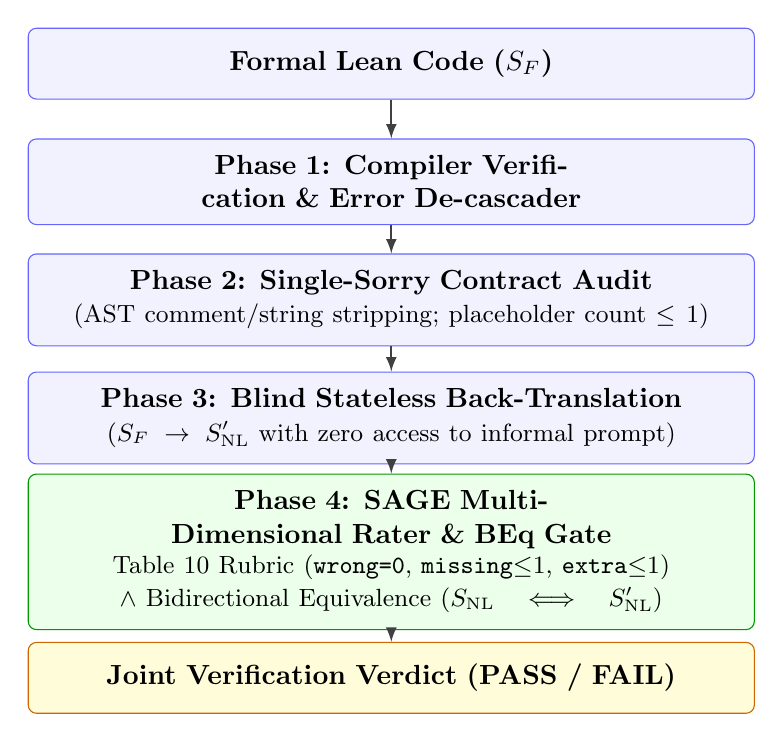
\begin{tikzpicture}[
    block/.style={rectangle, draw=blue!60, fill=blue!5, rounded corners=3pt, 
                  minimum height=0.9cm, text width=8.8cm, align=center, inner sep=6pt},
    gateblock/.style={rectangle, draw=green!60!black, fill=green!8, rounded corners=3pt, 
                      minimum height=1.1cm, text width=8.8cm, align=center, inner sep=6pt},
    verdictblock/.style={rectangle, draw=orange!80!black, fill=yellow!15, rounded corners=3pt, 
                         minimum height=0.9cm, text width=8.8cm, align=center, inner sep=6pt},
    arrow/.style={draw=black!75, -latex, thick}
]

    % Nodes positioned with clean vertical spacing
    \node [block] (source) at (0, 0) {
        \textbf{Formal Lean Code ($S_F$)}
    };

    \node [block] (compiler) at (0, -1.5) {
        \textbf{Phase 1: Compiler Verification \& Error De-cascader}\\
    };

    \node [block] (sorry) at (0, -3.0) {
        \textbf{Phase 2: Single-Sorry Contract Audit}\\
        \small (AST comment/string stripping; placeholder count $\le 1$)
    };

    \node [block] (back) at (0, -4.5) {
        \textbf{Phase 3: Blind Stateless Back-Translation}\\
        \small ($S_F \to S_{\text{NL}}'$ with zero access to informal prompt)
    };

    \node [gateblock] (gate) at (0, -6.2) {
        \textbf{Phase 4: SAGE Multi-Dimensional Rater \& BEq Gate}\\
        \small Table 10 Rubric (\texttt{wrong=0}, \texttt{missing}$\le$1, \texttt{extra}$\le$1) \\
        \small $\land$ Bidirectional Equivalence ($S_{\text{NL}} \iff S_{\text{NL}}'$)
    };

    \node [verdictblock] (verdict) at (0, -7.8) {
        \textbf{Joint Verification Verdict (PASS / FAIL)}
    };

    % Connecting Arrows
    \path [arrow] (source) -- (compiler);
    \path [arrow] (compiler) -- (sorry);
    \path [arrow] (sorry) -- (back);
    \path [arrow] (back) -- (gate);
    \path [arrow] (gate) -- (verdict);

\end{tikzpicture}
\caption{The SAGE Dual-Signal Bidirectional Verification Architecture.}
\label{fig:sage_architecture}
\end{figure}

The verification stages operate as follows:
\begin{itemize}
    \item \textbf{Phase 1 (Compiler Verification)}: Invokes \texttt{lake env lean}, isolating primary root-cause type errors from secondary cascades.
    \item \textbf{Phase 2 (Single-Sorry Contract)}: Strips all block comments (\texttt{/-\dots-/}), line comments (\texttt{--\dots}), and string literals to prevent AST spoofing, asserting that total placeholder axioms satisfy $\text{Count} \le 1$.
    \item \textbf{Phase 3 (Stateless Back-Translation)}: An independent reasoner reconstructs the formal Lean signature into rigorous mathematical English ($S_{\text{NL}}'$) without access to the original source prompt, eliminating confirmation bias.
    \item \textbf{Phase 4 (SAGE Table~10 Rater and Bidirectional Equivalence)}: Audits the reconstructed statement $S_{\text{NL}}'$ against the mathematical source $S_{\text{NL}}$ across seven standardized dimensions:
    \begin{itemize}
        \item \texttt{wrong = 0}: zero tolerance for false claims or inverted arrows;
        \item \texttt{missing $\le$ 1} and \texttt{extra $\le$ 1}: bounded tolerance for omitted or smuggled hypotheses;
        \item \texttt{exactness $\ge$ 1}, \texttt{naturality $\ge$ 3}, \texttt{descriptive\_precision $\ge$ 3}, \texttt{semantic\_match $\ge$ 4};
        \item \texttt{BEq}: strict two-way logical equivalence ($S_{\text{NL}} \implies S_{\text{NL}}'$ and $S_{\text{NL}}' \implies S_{\text{NL}}$).
    \end{itemize}
\end{itemize}

\subsubsection{Auditing the Milgram--Steenrod Formalization: Diagnosing Semantic Gaps}

Subjecting our Milgram--Steenrod formalization to the verification layer demonstrated the power of fail-closed semantic checking. While the Lean compiler accepted all 1,065 lines with exit code~0, SAGE's multi-dimensional rater isolated both verified strengths and critical specification gaps:

\begin{enumerate}[(i)]
    \item \textbf{Verified Algebraic Soundness (\texttt{wrong = 0}, \texttt{extra = 0})}:
    In \texttt{Core.lean}, the extension group $E$ uses the $+f$ product while $\tilde{G} = G \times EA$ uses the twisted $-f$ law \eqref{tildeG mult}. A reversed sign or transposed right action ($z_1 \cdot g_1$ instead of $z_1 \cdot g_2$) would fail to cancel the cocycle shift, leaving an erroneous $2f(g_1, g_2)$ residue. SAGE verified that the cocycle shifts cancel identically without smuggling simplifying assumptions (such as commutativity or trivial coefficients), awarding $\texttt{wrong} = 0$ and $\texttt{extra} = 0$.

    \item \textbf{Generalization Asymmetry and Domain Mutation in Lemma~1.1}:
    In \texttt{Lemma11.lean}, the formalization parameterized the parameter coordinate over an arbitrary abstract preorder $(P, \le)$ with arbitrary basepoints $p_0, p_1 \in P$, proving collision on arbitrary word lists. In the mathematical source, coordinates are strictly constrained to the geometric unit interval in semi-normal form ($0 \le t_1 \le \dots \le t_n \le 1$). 
    
    This triggered an immediate failure of Bidirectional Equivalence ($\text{BEq} = \text{False}$, $\texttt{semantic\_match} = 3 < 4$). Although the formal theorem implies the source claim by specializing $P \to [0, 1]$, \emph{the source statement about the unit interval does not imply the theorem for arbitrary preorders}. SAGE's fail-closed design strictly flags this domain mutation, certifying that an autoformalized theorem must not silently substitute a generalized carrier for the author's intended geometric domain without an explicit specialization theorem.

    \item \textbf{Presentation Morphism vs. Word Calculation in Lemma~2.3}:
    In \texttt{Core.lean}, the lifting map $\Pi$ was defined on raw word lists. SAGE flagged that while the local collision check \texttt{piLetter\_collision} is algebraically exact, the formalization omitted the quotient descent: it did not prove that $\Pi$ factors through \texttt{Quotient.lift} to define a genuine group homomorphism $\Pi : E\tilde{G} \to EE$ between the Milgram--Steenrod presented groups.

    \item \textbf{Helper Identity vs. Target Theorem in Theorem~2.2}:
    In \texttt{Theorem22.lean}, the code verified scalar cancellation ($s \cdot t / t = s$) on finite-support functions. However, SAGE caught that the file never formalized the actual null-homotopy function $H_s(\vec{g}, \vec{z}, \vec{t})$ or the vector collision equality $H_s(\vec{g}, \vec{z}, \vec{t}) = H_s(\vec{g}', \vec{z}', \vec{t}')$ on the group bundle, awarding $\texttt{exactness} = 0$ and $\texttt{missing} = 3$ for proving a supporting fiber identity in place of the topological theorem.
\end{enumerate}

These diagnostics demonstrate that semantic bidirectional auditing provides an essential bridge between machine-checked proofs and faithful mathematical communication, enforcing that formal code proves precisely what the mathematical paper asserts.

\subsection{}

\begin{thebibliography}{99}
\bibitem{Ja} Jain, P. (2025). Central Extensions of Topological Groups and the Cohomology of Classifying Spaces [Master's thesis, IISER, Pune]. IISER Pune Digital Repository. \url{https://dr.iiserpune.ac.in/handle/123456789/10020}. Downloadable copy: \url{https://drive.google.com/file/d/1aLrZeLQ014gvvikD1G2gADeI3FxpJ5ea/view?usp=drivesdk}

\bibitem{JJS} Jain, P., Joshi, R., \& Spallone, S. (2026). Central Extensions and Cohomology. arXiv preprint. arXiv:2307.14658. \url{https://arxiv.org/abs/2307.14658}


\bibitem{MCP} What is the Model Context Protocol (MCP)? (2026, August 2). Model Context Protocol. \url{https://modelcontextprotocol.io/docs/2026-07-28/getting-started/intro}

\bibitem{SAIR} SAIR Foundation. (n.d.). Open models for mathematics. SAIR Foundation. Retrieved November 15, 2026, from \url{https://sair.foundation/open-math-model}

\bibitem{SAGE} Hirtz, T., Jafarrahmani, F., Sagueni, A., Zhou, X., Deng, W., \& Zhang, L. (2026). Sage: Formalization with Semantic Correction. \emph{arXiv preprint arXiv:2609.35790}. \url{https://arxiv.org/abs/2609.35790}

% \bibitem{AdMi} Adem, A. \& Milgram, R. J. (2004). Cohomology of Finite Groups (2nd ed.). Springer-Verlag.

% \bibitem{BoWa} Borel, A., \& Wallach, N. R. (2000). Continuous Cohomology, Discrete Subgroups, and Representations of Reductive Groups. Amer. Math. Soc.

% \bibitem{Br} Brown, R. (2006). Topology and Groupoids, published online at \url{groupoids.org.uk}. PDF available at \url{https://groupoids.org.uk/pdffiles/topgrpds-e.pdf}.

% \bibitem{Di} tom Dieck, T. (2008). Algebraic Topology. EMS Textbooks in Math.

% \bibitem{DuFo} Dummit, D. S., \& Foote, R. M. (2004). Abstract Algebra (3rd ed.). John Wiley \& Sons.

% \bibitem{EiMa} Eilenberg, S., \& MacLane, S. (1947). Cohomology Theory in Abstract Groups. I. Annals of Math., 48(1), 51–78. \url{https://doi.org/10.2307/1969215}

% \bibitem{FuWo}Fuchssteiner, M., \& Wockel, C. (2012). Topological Group Cohomology with Loop Contractible Coefficients. Topology and its App., 159(10-11), 2627-2634. \url{https://doi.org/10.1016/j.topol.2012.04.006}

% \bibitem{Ha} Hatcher, A. (2002). Algebraic Topology. Cambridge Uni. Press. \url{https://pi.math.cornell.edu/~hatcher/AT/ATpage.html}

% \bibitem{JoSp} Joshi, R., \& Spallone, S. (2023). Central Extensions and Cohomology. arXiv preprint. arXiv:2307.14658v2. \url{https://arxiv.org/abs/2307.14658v2}

% \bibitem{Mi} Milgram, R. J. (1967). The Bar Construction and Abelian H-spaces. Illinois J. Math., 11(2), 242-250. \url{https://doi.org/10.1215/ijm/1256054662}

% \bibitem{PiSp} Piccinini, R. A., \& Spreafico, M. (1998). The Milgram--Steenrod Construction of Classifying Spaces for Topological Groups. Exposition. Math., 16(2):97–130.

% \bibitem{Pu} Puppe, D. (1967). Bemerkungen über die Erweiterung von Homotopien. Archiv der Mathematik, 18, 81-88. \url{https://doi.org/10.1007/BF01899475}

% \bibitem{A1} Stasheff, J. D. (1963). Homotopy Associativity of H-Spaces. I. Trans. Amer. Math. Soc., 108(2), 275–292. \url{https://doi.org/10.2307/1993608}

% \bibitem{A2} Stasheff, J. D. (1963). Homotopy Associativity of H-Spaces. II. Trans. Amer. Math. Soc., 108(2), 293–312. \url{https://doi.org/10.2307/1993609}

% \bibitem{Stash} Stasheff, J.D. (1978). Continuous Cohomology of Groups and Classifying Spaces. Bull. Amer. Math. Soc., 84(4), 513-530. \url{https://www.ams.org/journals/bull/1978-84-04/S0002-9904-1978-14488-7/}

% \bibitem{St} Steenrod, N. E. (1968). Milgram's Classifying Space of a Topological Group. Topology, 7(4), 349-368. \url{https://core.ac.uk/download/pdf/82066845.pdf}

% \bibitem{Strickland} Strickland, N. P. (2009). The Category of CGWH Spaces. preprint. \url{https://ncatlab.org/nlab/files/StricklandCGHWSpaces.pdf}

% \bibitem{WaWo} Wagemann, F., \& Wockel, C. (2015). A Cocycle Model for Topological and Lie Group Cohomology. Trans. Amer. Math. Soc., 367(3), 1871-1909. \url{https://www.jstor.org/stable/24513021}

% \bibitem{We} Weibel, C. A. (1994). An Introduction to Homological Algebra. Cambridge Uni. Press.

% \bibitem{Wi} Wigner, D. (1973). Algebraic Cohomology of Topological Groups. Trans. Amer. Math. Soc., 178, 83-93. \url{https://egg.epfl.ch/~nmonod/bonn/Wigner_1973.pdf}

% \bibitem{Dirty} Tyler Lawson (2009). ``Dirty" proof that Eilenberg-MacLane spaces represent cohomology?. MathOverflow. \url{https://mathoverflow.net/q/5521} (version: 14 Nov. 2009)

% \bibitem{nlab1} nLab authors (2025, January). colimits of paracompact Hausdorff spaces. \url{https://ncatlab.org/nlab/show/colimits+of+paracompact+Hausdorff+spaces}, \href{https://ncatlab.org/nlab/revision/colimits+of+paracompact+Hausdorff+spaces/14}{Revision 14}


        
\end{thebibliography}

\end{document}
